% !TEX root = paper.tex
\section{Background and Motivation}
\label{sec:motivation}

\subsection{Automatic DOALL Software-only Systems}

\begin{table*}
  % !TEX root = ../paper.tex
\newcommand{\sbcheck}{\textcolor{ForestGreen}{\ding{51}}}
\newcommand{\sbcross}{\textcolor{RubineRed}{\ding{55}}}
\small
\centering
\begin{tabular}{|l|c|c|c|c|c|c|c|c|c|}
\hline
\multirow{2}{*}{Technique}   &
% \multirow{2}{*}{\parbox[c]{1.1cm}{\centering Fully\\ Automatic}} &
\multirow{2}{*}{\parbox[c]{1cm}{\centering Supports \\Spec}} &
\multirow{2}{*}{\parbox[c]{1.8cm}{\centering Supports Ptrs \\ and DynAlloc}} &
\multicolumn{2}{c|}{Supports Privatization} &
\multicolumn{2}{c|}{Supports Reduction} &
\multirow{2}{*}{\parbox[c]{1.4cm}{\centering Efficient \\Privatization}} &
\multirow{2}{*}{\parbox[c]{0.6cm}{\centering Cheap \\ Spec}} &
\multirow{2}{*}{\parbox[c]{1.7cm}{\centering \# Cores \\ Evaluated on}} \\

\cline{4-7}
&  &
& \parbox[c]{1cm}{\centering Static}   & \parbox[c]{1cm}{\centering Spec}
& \parbox[c]{1cm}{\centering Static} & \parbox[c]{1cm}{\centering Spec}
& & & \\ \hline

%%% LRPD %%%
\parbox[l]{2.4cm}{LRPD \cite{rauchwerger:95:sigplan,dang:02:ipdps}} & \sbcheck  & \sbcross & ?  & \sbcheck    & ?  & \sbcheck   & \sbcross    & \sbcross    & 14    \\ \hline

%%% Polaris %%%
\parbox[l]{2.4cm}{Polaris \cite{tu:94:lcpc,blume:96:icpp}} & \sbcross & \sbcross & \sbcheck    & \sbcross   & \sbcheck   & \sbcross  & \sbcheck    & \sbcross    & 8  \\ \hline

%%% SUIF %%%
\parbox[l]{2.4cm}{SUIF \cite{suif:94:stanford,hall:05:toplas}} & \sbcross & \sbcross & \sbcheck   & \sbcross   & \sbcheck  & \sbcross  & \sbcross    & \sbcross    & 4, 8   \\ \hline


%%% Sensitivity %%%
\parbox[l]{2.4cm}{Sensitivity \cite{Rus:07:ics}}  & \sbcheck  & \sbcross & \sbcheck    & \sbcheck    & \sbcheck   & \sbcheck   & \sbcheck     & ?    & 4 \\ \hline


%%% STMLite %%%
\parbox[l]{2.4cm} {STMLite \cite{mehrara:09:stmlite}} & \sbcheck  & \sbcheck  & \sbcheck   & \sbcheck   & \sbcross  & \sbcross  & \sbcross    & \sbcross    & 8 \\ \hline

% %%% Array Privatization %%%
% \parbox[l]{1.9cm}{Array \\Privatization\\ (Tu \& Padua)} & \sbcheck  & \sbcross & \sbcross & \sbcheck    & \sbcross   & \sbcross  & \sbcross  & \sbcheck     & \sbcross    & 8?    \\ \hline

%%% ClusterDOALL %%%
\parbox[l]{2.4cm}{ClusterDOALL \cite{kim:12:cgo}}  & \sbcheck  & \sbcheck  & \sbcross   & \sbcheck    & \sbcross  & \sbcross  & \sbcross & \sbcheck     & 120   \\ \hline

%%% Privateer %%%
\parbox[l]{2.4cm}{Privateer \cite{johnson:12:pldi}}  & \sbcheck  & \sbcheck  & \sbcross   & \sbcheck    & \sbcross  & \sbcheck   & \sbcross & \sbcheck     & 24    \\ \hline

%%% LSD %%%
\parbox[l]{2.4cm}{LSD (This work)} & \sbcheck  & \sbcheck  & \sbcheck    & \sbcheck    & \sbcheck   & \sbcheck   & \sbcheck     & \sbcheck     & 28    \\ \hline
\end{tabular}
  \caption{
    Comparison of LSD with Automatic DOALL software-only systems.
  }
  \label{tab:related-work}
    \vspace{-5pt}
\end{table*}

\begin{figure}
  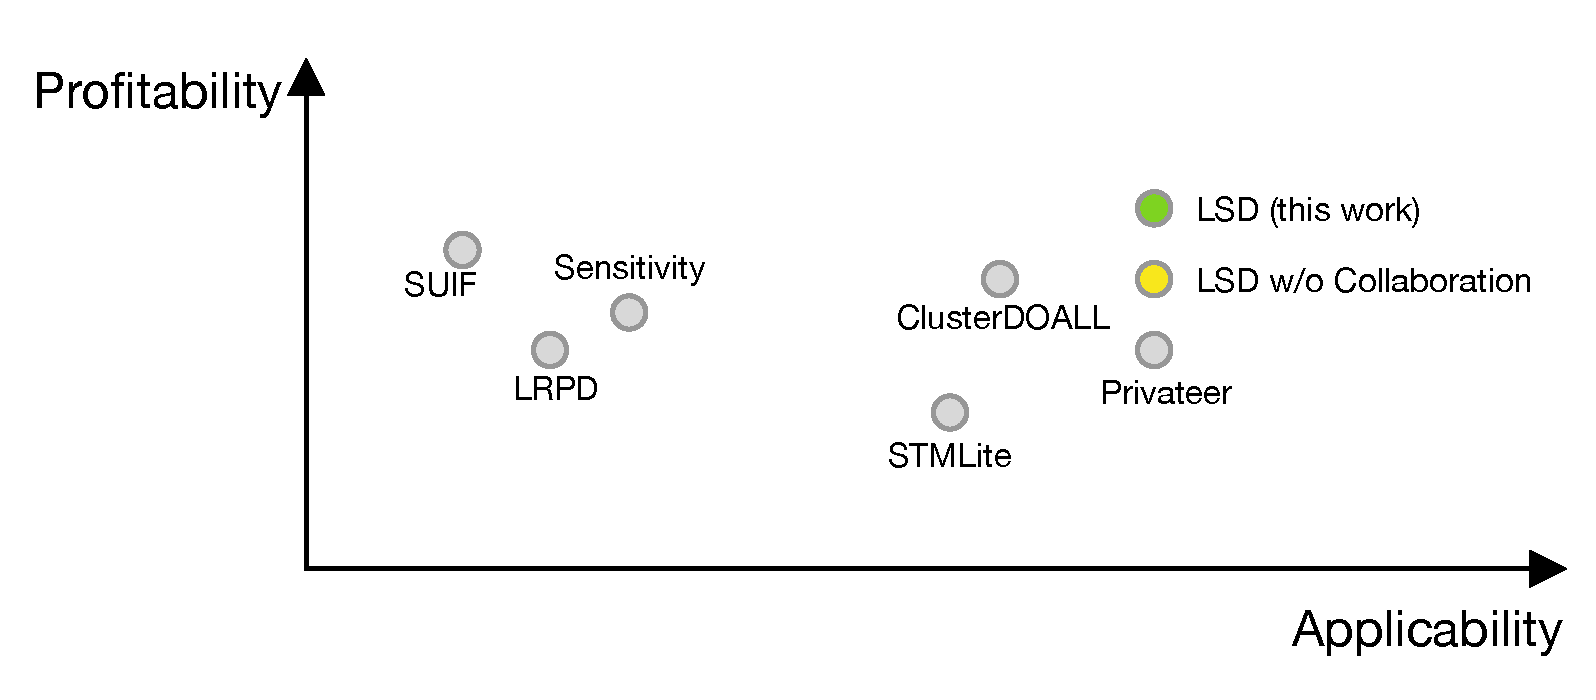
\includegraphics[width=\columnwidth]{figures/profit-appli-compare}
  \caption{Comparison of applicability and profitability.}
  \label{fig:profit-appli-compare}
\end{figure}


\subsection{DOALL parallelization}

In DOALL parallelization, loop iterations need to run independently of each
other.  There cannot be any loop-carried (cross-iteration) memory flows (RAW
dependences), unless a reduction is identified. Loop-carried false and anti (WAW
and WAR) memory dependences need to be handled by privatization or reduction.
At the end of parallel invocation, workers need to merge their memory states to
a single live-out memory state.  Merging reduction objects is inexpensive and
does not require bookkeeping during the parallel invocation.  Merging private
objects though can be very expensive. For every memory location of private
objects the last written value needs to be determined. If it cannot be
determined statically, then it needs to be tracked dynamically, resulting in
significant bookkeeping for all the involved stores.




%Many proposals speculate low-level properties of the code, namely dependences
%between individual operations.
%%
%Such speculative systems work well when assisted by hardware
%extensions~\cite{TLS_papers...}, but yield small speedups, if any, when
%running on commodity hardware.
%%TODO: other software-spec apart from STM, more recent ones ??
%For example, Software Transactional Memories
%(STMs)~\cite{mehrara:09:stmlite} present an abstraction that facilitates
%speculating the independence of memory transactions (i.e., memory
%speculation). Validation requires logging or communication for most of the
%memory accesses within each transaction and becomes prohibitively expensive
%as the size of transaction grows.
%%
%%This reduces to comparing the read and write sets of adjacent transactions.  As
%%transactions grow, the number of memory operations within that transaction can
%%become prohibitively large. Further, instrumenting every memory operation with
%%the transaction to log or communicate every access---approximately one tenth of
%%all dynamic instructions---leads to an excessive overhead, even in the absence
%%of transaction rollbacks.
%
%%privateer
%
%%An alternative approach is to reduce memory
%
%
%Other speculative systems attempt to avoid the excessive memory speculation of
%generic transactional systems by speculating higher-level properties whose
%validation does not require logging or communication.
%%
%A prominent work of this class is Privateer~\cite{johnson:12:pldi:short}, a
%state-of-the-art Spec-DOALL parallelization system, that exhibits more
%scalable speedups compared to prior work.
%%
%Privateer partitions memory objects into several categories/families according
%to observed access patterns via profiling.  Speculating that certain
%individual memory access pairs are independent is avoided by just speculating
%separation of the families and some other simple properties.  However, detection
%of privatizable memory objects relies solely on memory and control profiling.
%Therefore, validation for a substantial set of memory objects still requires
%expensive logging and checks at every memory access, similarly to STM systems.
%% and occassional communication among workers
%%cheap spec for short-lived or read-only has also been discussed in other spec
%%systems such as cluster-doall and corD
%%

%STMLite, privateer, LRPD, ClusterDoall,
%Polaris, CorD, SUIF
%
%use of static analysis
%
%cheap spec techniques usage
%
%privatization support
%
%handling c/c++ complex data structures, pointers
%
%privatization cost
%
%reductions support
%
%scalable results (cores used)

%Table 1 compares thiswork with other existing automatic parallelization systems.
%Table ~\ref{related_work} summarizes comparison with prior work.


\subsubsection{Analysis-based Approaches}

static analysis limitations

Efforts to augment static analysis with low-cost run-time analysis are limited
to simple cases where a predicate can be extracted outside the loop of
interest~\cite{hybrid_analysis, suif:94:stanford, polaris}.
%TODO: check if it is only affine loops for hybrid. that's the case for suif and
%polaris
%
%the dependence patterns of real applications are frequently driven by the
%program input, or experience a phase change during program execution
Overall, current analysis-based parallelizing
compilers~\cite{campanoni:2012:iscgo, raman:2008:iscgo, suif:94:stanford,
polaris, sensitivity} when applicable can deliver good predictable speedups, but
they all suffer from the aforementioned limitations, and consequently fail to
enable aggressive and scalable parallelization for most general-purpose
applications.


\subsection{Motivational example}

This work is motivated by the excessive use of memory speculation and expensive
privatization of prior speculative systems that limited their efficiency.
%
In this section, we present a code example taken from MiBench~\cite{} benchmark
dijkstra (used in the evaluation of Privateer~\cite{}) to showcase how static
analysis along with cheap-to-validate speculative assumptions can infer
high-level program properties and enable scalable parallelization.
%
We focus on two memory objects that would cause inefficiencies on prior
parallelization systems.
%
For each of these objects, we examine how we can tackle DOALL parallelization
inhibitors; in particular loop-carried memory dependences, and exhibit the
multiplicative effect of collaboration in terms of analysis accuracy.

First, a quick description of the used static and speculative analyses in our
example:
%
\begin{itemize}
%
\item \textit{Static Analysis} (see ~\cite{johnson:17:cgo} for more information)
%
  \begin{itemize}
%
  \item \textit{Alias Analysis}: an ensemble of analysis algorithms that
determine whether the footprint of an operation alias the footprint of another
operation.
%
  \item \textit{Kill-Flow}: searches for killing operations along all feasible
paths between two operations. It searches blocks which post-dominate the source
of the queried dependence and dominate the destination.
%
  \item \textit{No-Capture Source}: identifies global variables or allocators
whose address is never captured. Such objects can only be referenced through
addresses computed from the object's name. The algorithm, thus, can enumerate,
transitively, all uses of that object.
%
\end{itemize}
%
\item \textit{Speculative Analysis}
%
\begin{itemize}
%
  %\item \textit{Loop-Invariant Loaded Value Prediction}:
  \item \textit{Value Prediction Speculation~\cite{}}: identifies, using
value-prediction, profiling the predictable outcome of certain instructions.
%cite F.  Gabbay  and  A.  Mendelson.    Can  program  profiling  supportvalue
%prediction?
%
  \item \textit{Control Speculation~\cite{}}: identifies, using edge profiling,
speculatively dead code and asserts absence of memory dependences to or from
speculatively dead operations.
%cite W. Y. Chen, S. A. Mahlke, and W. W. Hwu.  Tolerating first levelmemory
%access latency in high-performance systems
%
\end{itemize}
%
\end{itemize}
%

\lstset{basicstyle=\ttfamily, numbers=left, numberstyle=\tiny,
  stepnumber=1, numbersep=5pt}
\begin{figure*}[t]
  \centering
  \scriptsize
  \subfloat[dijkstra]
  {
    \label{fig:dijkstra}
    \begin{minipage}{7.5cm}
      \begin{lstlisting}[morekeywords={iPrev,piPrev,g_qCount},belowskip=0pt]
// global variables
int iPrev;
int g_qCount = 0;

void enqueue(..., int piPrev) {
  ...
  ... = piPrev;
  g_qCount++;
}

void dequeue(..., int *piPrev) {
  if (qHead) {
    ...
    *piPrev = ...
    g_qCount--;
  }
}

for (int i = 0; i < N; i++) { // hot loop
  ...
  enqueue(i, 0, NONE);
  while ( g_qCount ) {
    dequeue(&iNode, &iDist, &iPrev);
    for (k = 0; k < NUM_NODES; k++) {
      ...
      if ( valid node ) {
        ...
        enqueue(i, iDist+iCost, iNode);
      }
    }
  }
  ...
}

\end{lstlisting}

    \end{minipage}
  }
\end{figure*}

%showcases how fine-grained collaboration between static analysis and speculative
%assumptions can infer high-level program properties without the need for
%expensive memory speculation.

%Dependence has three conditions. We say there is a memorydependence  from
%instructioni1to  instructioni2iff(alias)the footprint of operationi1may-aliasthe
%footprint ofi2, and(feasible-path) there is a feasible path of execution
%fromi1toi2which (no-kill) does not contain an operation which over-writes the
%common memory footprint. Footprint denotes theset of memory locations read or
%written by the instruction.

1) global object \textit{g\_qCount}

\textbf{Static analysis and inexpensive speculation in isolation}:
%
%Analysis Results:
Static analysis cannot disprove all loop-carried RAW and WAW dependences on
accesses of g\_qCount.
%
Profile information indicates that the first load of g\_qCount in each iteration
always returns zero.  Using this information, value prediction removes the
loop-carried RAW dependence sinking on this load.
%
Removal of this dependence prevents usage of memory speculation for this
particular load.
%
Presence of WAW dependences though necessitates privatization of the memory
object, and value prediction cannot reason about store instructions and cannot
give any additional information related to output dependences.
%
%Cost
The cost in this case includes the validation overhead for value prediction
(perform load before loop exits or on backedges and compared predicted value
with loaded value) and the privatizaition cost (monitor stores participating in
the WAW dependences to determine last written value). Bookkeping for
privatization is the dominant cost as it requires updating metadata multiple
times per loop iteration (given that some stores are within inner loops).
%dynamic resolution to determine last written value


\textbf{Collaboration of static and speculative analysis}:
%
This value prediction can be seen as a store before the first load of g\_qCount
that kills any data flow for this memory object from previous iterations.
%
An extended speculative analysis removes, similarly to the first case, the
loop-carried RAW dependence, but additionally queries alias analysis for
must-aliasing accesses with the load's address. If these accesses are dominated
by the load, then loop-carried RAW or WAW dependences from or to these accesses
can be ignored.
%
This remvoes the need to perform dynamic resolution of the last written value;
the final content of this memory location is predictable.
%any action to log (for last write) any of these individual memory operations.
%
%Interestingly, this case of privatization goes beyond the classical definition
%of privatization definition~\cite{tu-padua-array-privatization-1994}  that
%requires that every load of a privatizable element is preceded by a store to
%the element in the same iteration of the loop. In this scenario, global
%variable g\_qCount is first loaded at every iteration, a data flow exists.
%
%
The cost in this case only includes the small validation overhead for value
prediction. There is no bookkeping cost for privatization.
%
No prior work could detect and so effectively handle this new case of
privatization.
%- privatization cost: none avoid dynamic resolution to determine last written
%value (live-out value)

%TODO: use this first
2) global object \textit{iPrev}

- speculative assumption: the branch "if (qHead)" is always taken (control speculation)

- static analysis: alias analysis, killflow, noCaptureGlobal analysis passes

- validation cost: no validation cost for control spec (just misspecs if branch
  is not taken)

- Using the speculative assumption, killflow analysis can infer that the store
  in line 15 kills all other accesses of this global
variable (killed operations are identified by quering alias analysis). Given this
property, any RAW loop-carried dependence is disproved.  Additionally, static
analysis can enumerate all uses of this global, since it is not captured, and
detect that this global is used only within this loop, namely it is not a
live-out.  Thus, there is no need to log stores and keep track of the last
written value to it.

%3) TODO: example with blackscholes

For all the above memory objects, Privateer~\cite{}, the state-of-the-art DOALL
system that we mainly compare against, would require expensive logging on most
of their accesses,
%either for validation checks or for identifying who wrote last what
yielding sub-optimal speedups as clearly exhibited by our experimental results
in section ~\ref{eval}.
%all these objects are classified as privatizable by Privateer

Note that our framework is not limited to static global allocations.  It can
handle linked or recursive data structures, pointers,type  casts,  and  dynamic
allocation.

%use alvinn for value pred + alias analysis

%Note that WAR dependences can be ignored thanks to the process-based runtime
%system.


\centering
\tiny
\begin{tabular}{|c|c|c|c|c|c|c|c|c|}
  \hline
  Type of Private &
  Overlap         &
  Spec Privatization &
  Other Spec Allowed    &
  Loads Checks  &
  Store Checks    &
  Last-Write Detection &
  CoW Mapping &
  Copy-out to Main \\

%%%%%%%%%%%%%%%%%%% Shared %%%%%%%%%%%%%%%%%%%%%%%%%%
 \hline
 Shared & No & - & - & - & - & - & - & - \\
 \hline
%%%%%%%%%%%%%%%%%%% Local %%%%%%%%%%%%%%%%%%%%%%%%%%
 Local Private & Any & - & $\checkmark$ & - & - & - & $\checkmark$ & - \\
 \hline
%%%%%%%%%%%%%%%%%%% Overwrite %%%%%%%%%%%%%%%%%%%%%%%%%%
 Kill Private & Complete & - & $\checkmark$ & - & - & - & $\checkmark$ &
$\checkmark$ \\
 \hline
%%%%%%%%%%%%%%%%%%% Conservative Private %%%%%%%%%%%%%%%%%%%%%%%%%%
 Static Private & No/Partial & - & $\checkmark$ & - & - &
 $\checkmark$ & $\checkmark$ & $\checkmark$ \\
 \hline
%%%%%%%%%%%%%%%%%%% Specpriv Private %%%%%%%%%%%%%%%%%%%%%%%%%%
 Privateer Private & Any & $\checkmark$ & $\checkmark$ & $\checkmark$ & $\checkmark$ &
 $\checkmark$ & $\checkmark$ & $\checkmark$ \\
 \hline
\end{tabular}



%\lstset{basicstyle=\ttfamily, numbers=left, numberstyle=\tiny,
%  stepnumber=1, numbersep=5pt}
%\begin{figure*}[t]
%  \centering
%  \scriptsize
%  \subfloat[dijkstra -- predictable]
%  {
%    \label{fig:dijkstra}
%    \begin{minipage}{7.5cm}
%      \begin{lstlisting}[morekeywords={g_qCount},belowskip=0pt]
// predicted to be 0 at start of every iteration
int g_qCount = 0;

for ( int i = 0; int j = N/2; i < N; i++, j++ ) {
  ...
  enqueue( i, 0, NONE );
  g_qCount++;
  while ( g_qCount ) {
    dequeue( &iNode, &iDist, &iPrev );
    g_qCount--;
    for ( k = 0; k < NUM_NODES; k++ ) {
      ...
      if ( valid_node ) {
        ...
        enqueue( i, iDist + iCost, iNode );
        g_qCount++;
      }
    }
  }
  ...
}

\end{lstlisting}

%    \end{minipage}
%  }
%  \hspace{0.5cm}
%  \subfloat[dijkstra -- overwrite]
%  {
%    \label{fig:blackscholes}
%    \begin{minipage}{7.5cm}
%      \input{figures/dijkstra_overwrite_code}
%    \end{minipage}
%  }
%\end{figure*}
%
%
%
%
%\begin{figure*}[t]
%  \centering
%  \scriptsize
%  \subfloat[gemm -- shared]
%  {
%    \label{fig:gemm}
%    \begin{minipage}{7.5cm}
%      \begin{lstlisting}[escapeinside={~}{~}, belowskip=0pt]
for ( i = 0; i < ni; i++ ) {
  for ( j = 0; j < nj; j++ ) {
    C[i][j] *= beta; 
    for ( k = 0; k < nk; ++k )
      C[i][j] += alpha * A[i][k] * B[k][j];
  }
}
\end{lstlisting}

%    \end{minipage}
%  }
%  \hspace{0.5cm}
%  \subfloat[blackscholes -- overwrite]
%  {
%    \label{fig:blackscholes}
%    \begin{minipage}{7.5cm}
%      % look in Nick's motivation.tex for formatting
\begin{lstlisting}[morekeywords={prices}, belowskip=0pt]
for ( j = 0; j < NUM_RUNS; j++ ) {
  for ( i = 0; i < numOptions; i++ ) {
    prices[i] = BlkSchlsEqEuroNoDiv(
      sptprice[i], strike[i],
      rate[i], volatility[i], otime[i],
      otype[i], 0);
  }
}
\end{lstlisting}

%    \end{minipage}
%  }
%\end{figure*}
%\begin{figure*}[t]
%  \centering
%  \scriptsize
%  \subfloat[052.alvinn -- stack local]
%  {
%    \label{fig:alvinn_local}
%    \begin{minipage}{7.5cm}
%      \begin{lstlisting}[morekeywords={psum_array},belowskip=0pt]
float psum_array[NHU+1]; // stack

for (epoch = 0; epoch < NUM_EPOCHS; epoch++) {
  ...
  for ( i = 0; i < NHU+1; i++ )
    psum_array[i] = 0;
  for( i = 0; i < NOU; i++ ) {
    for ( j = 0; j < NHU+1; j++ ) {
      ...
      psum_array[j] += delta[i] * weights[i][j];
      ...
    }
  }
  for ( i = 0; i < NHU+1; i++ )
    delta[i] = hidden[i] * (1 - hidden[i]) * psum_array[i];
  ...
}
\end{lstlisting}

%    \end{minipage}
%  }
%  \hspace{0.5cm}
%  \subfloat[dijkstra -- global local]
%  {
%    \label{fig:dijkstra}
%    \begin{minipage}{7.5cm}
%      \begin{lstlisting}[morekeywords={k},belowskip=0pt]
int k;

for ( int i = 0; int j = N/2; i < N; i++, j++ ) {
  ...
  j = j%N;
  if ( i == j )
    continue;
  else {
    ...
    while ( g_qCount ) {
      ...
      for ( k = 0; k < NUM_NODES; k++ ) {
        ...
      }
    }
  }
  ...
}

\end{lstlisting}

%    \end{minipage}
%  }
%\end{figure*}

% \begin{figure*}[t]
%   \centering
%   \scriptsize
%   \subfloat[covariance -- nospec-private]
%   {
%     \label{fig:covariance}
%     \begin{minipage}{7.5cm}
%       \begin{lstlisting}[morekeywords={symmat}, belowskip=0pt]
for ( j1 = 0; j1 < m; j1++ ) {
  for ( j2 = j1; j2 < m; j2++ ) {
    symmat[j1][j2] = 0.0;
    for ( i = 0; i < n; i++ )
      symmat[j1][j2] += data[i][j1] * data[i][j2];
    symmat[j2][j1] = symmat[j1][j2];
  }
}
\end{lstlisting}

%     \end{minipage}
%   }
%   \hspace{0.5cm}
%   \subfloat[052.alvinn -- real private]
%   {
%     \label{fig:alvinn_specpriv}
%     \begin{minipage}{7.5cm}
%       \begin{lstlisting}[morekeywords={output_act}, belowskip=0pt]
float output_act[NOU];

for (epoch = 0; epoch < NUM_EPOCHS; epoch++) {
  ...
  receiver = &output_act[0];
  end_receiver = &output_act[NOU - 1];
  for ( ; receiver <= end_receiver; ) {
    *receiver = 0.0;
    sender = &hidden_act[0];
    end_sender= &hidden_act[NHU];
    for (; sender <= end_sender; )
      *receiver += (*sender++) * (*weight++);
    *receiver = SIGMOID(*receiver);
    *receiver++;
  }
  ...
  for (ou = 0; ou < NOU; ou++) {
  	delta[ou] = (teach[ou] - output_act[ou]) *
      output_act[ou] * (1.0 - output_act[ou]);
  	...
  }
  ...
}
\end{lstlisting}

%     \end{minipage}
%   }
% \end{figure*}
